\documentclass[11pt]{article}
\usepackage{icmlko}
\begin{document}

\title{집단 표지가 공유 축을 풀어 준다 --- 안 덮은 도메인이 제일 벌었다}
\author{월드모델 실험실}
\date{노트 413 · 2026년 8월 2일}
\maketitle

\begin{abstract}
노트 412가 시장팝업 전용 축에서 값을 찾았지만 판에 못 실었다 --- 표적은
$+0.0241$ 인데 아이돌이 $-0.0115$ 로 냈다. 진단은 \emph{전용 축은 남에게
상수 열이고 그 도메인 원핫과 공선이라 과적합 연료가 된다} 였다.

같은 서랍을 더 열었다. \texttt{lab/grpaxes.py} 의 \textbf{grp} --- 노트 138이
바닥선을 만들려고 지은 집단 표지 축인데 \textbf{챔피언에 한 번도 안 들어가
있었다.} 여덟 도메인에 $100\%$ 덮음이고 전부 기획 시점 정보다(연령등급 ·
무료 여부 · 매체 · 포맷 · 국가 · 카테고리).

노트 412의 진단을 그대로 사전 등록에 옮겼다 --- \emph{덮인 여덟이 벌고
안 덮인 셋(아이돌 · 팝업 · 시장팝업)이 낸다.}

\begin{center}
\begin{tabular}{lrr}
\hline
짝 12뽑기, grp 넣기 & 평균 이득 & \\
\hline
덮인 여덟 & $+0.0042$ & \\
\textbf{안 덮인 셋} & $\mathbf{+0.0278}$ & 아이돌 $+0.0482$ · 팝업 $+0.0361$ \\
\hline
\textbf{판} & $\mathbf{+0.0029 \pm 0.0025}$ & $\mathbf{11/12}$ \\
\hline
\end{tabular}
\end{center}

\textbf{사전 등록이 거꾸로 틀렸다.} 안 덮인 도메인이 덮인 도메인의
\textbf{여섯 배}를 벌었다. 조건 ①(부호 $11/12$)로 \textbf{채택}했다 ---
씨앗 12평균 판 $0.4659 \to \mathbf{0.4696 \pm 0.0004}$, 분모 3{,}430 그대로.
\end{abstract}

\section{왜 안 덮인 쪽이 버나}

grp 가 없을 때 나무는 \textbf{공유 축으로 도메인을 갈라야} 한다 --- 어떤
축이 어느 도메인에서 어떻게 작동하는지를 축 자체로 배워야 하고, 그러느라
축이 도메인 \emph{안}의 신호를 나르는 데 덜 쓰인다. grp 를 주면 나무가
\textbf{도메인 사이 분산을 그 열 하나로 흡수}하고 공유 축은 도메인 안에서
일하게 된다.

그 이득은 \textbf{공유 축에 제일 많이 기대던 도메인}에게 간다. 아이돌은
전용 축이 거의 없고(노트 410: 선형 $\rho$ 가 $-0.0295$ 라 신호가 전부
비선형) 팝업은 관측 축이 다섯뿐이다. \textbf{둘 다 grp 가 안 덮는데 제일
크게 번다.}

\section{노트 412의 진단은 법칙이 아니었다}

\texttt{mkt} 축 다섯은 남들에게 해가 됐고(아이돌 $-0.0115$),
\texttt{grp} 하나는 남들에게 득이 됐다(아이돌 $+0.0482$). 둘 다 안 덮는
도메인에 중립 $0.5$ · 표시자 $0$ 이 들어간다. 차이는 \textbf{그 열이
실제로 일을 하느냐}다 --- mkt 는 열한 중 \textbf{하나}에서만 값이 있어
사실상 ``시장팝업이냐''를 다섯 번 더 묻는 열이었고, grp 는 열한 중
\textbf{여덟}에서 값이 있어 진짜 자질이다.

\textbf{그래서 규칙은 ``전용 축은 안 된다''가 아니라 ``한 도메인만 아는
열은 이름표를 한 번 더 적는 것''이다.}

\section{creator\_track 은 중복이었다}

같이 시험한 팔 C(grp $+$ creator\_track $+$ anime\_medium)는 판
$+0.0010 \cdot 6/12$ 로 내려앉는다. 사전 등록에 미리 적어 뒀다 --- 노트 164가
\texttt{venue\_prominence} 슬롯이 일곱 도메인에서 \textbf{실은 제작 주체의
사전 출시작 수}라고 밝혔으니 creator\_track 은 그 일곱에서 같은 것을 두 번
넣는 셈이다. \textbf{grp 만 넣는다.}

\section{웹툰, 네 번째}

웹툰은 여기서도 혼자 크게 낸다($-0.0087 \cdot 0/12$). 깊이(노트 406) ·
lr(노트 408) · 자루 섞기(노트 409)에 이어 \textbf{네 번째로 같은 자리에
혼자 있다.} 판 무게 $21\%$ 짜리가 매번 반대편에 선다.

\begin{tabular}{lp{7.2cm}}
\hline
웹툰 & 네 번 연속 유일한 체계적 손실. 이제는 이것 자체가 재야 할 대상이다 \\
전용 축의 통로 & 시장팝업 $+0.0241$ 은 아직 갈 곳이 없다. owning 도메인에만
보이는 2단이 남은 후보 \\
서랍 & grp 가 이렇게 오래 안 쓰였다면 다른 것도 있다 \\
\hline
\end{tabular}

\begin{figure}[h]
\centering
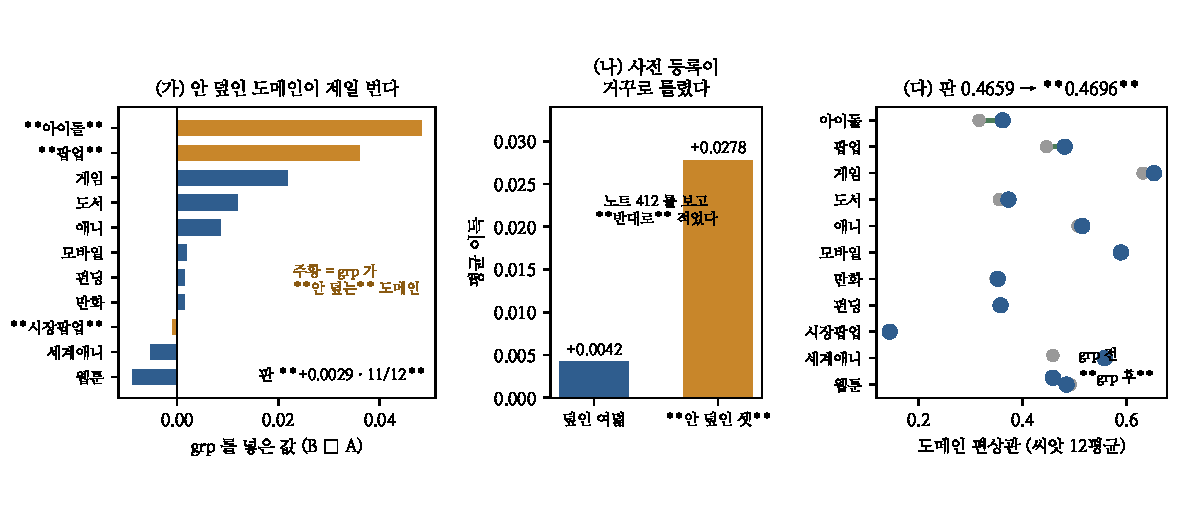
\includegraphics[width=\textwidth]{figs/fig413.pdf}
\caption{(가) 도메인별 이득 --- 주황이 grp 가 안 덮는 셋. (나) 사전 등록이
거꾸로 틀렸다. (다) 채택 뒤 판 $0.4659 \to 0.4696$.}
\end{figure}

\end{document}
